\documentclass[ignorenonframetext,]{beamer}
\setbeamertemplate{caption}[numbered]
\setbeamertemplate{caption label separator}{: }
\setbeamercolor{caption name}{fg=normal text.fg}
\beamertemplatenavigationsymbolsempty
\usepackage{lmodern}
\usepackage{amssymb,amsmath}
\usepackage{ifxetex,ifluatex}
\usepackage{fixltx2e} % provides \textsubscript
\ifnum 0\ifxetex 1\fi\ifluatex 1\fi=0 % if pdftex
  \usepackage[T1]{fontenc}
  \usepackage[utf8]{inputenc}
\else % if luatex or xelatex
  \ifxetex
    \usepackage{mathspec}
  \else
    \usepackage{fontspec}
  \fi
  \defaultfontfeatures{Ligatures=TeX,Scale=MatchLowercase}
\fi
\usetheme[]{AnnArbor}
\usecolortheme{dolphin}
\usefonttheme{professionalfonts}
% use upquote if available, for straight quotes in verbatim environments
\IfFileExists{upquote.sty}{\usepackage{upquote}}{}
% use microtype if available
\IfFileExists{microtype.sty}{%
\usepackage{microtype}
\UseMicrotypeSet[protrusion]{basicmath} % disable protrusion for tt fonts
}{}
\newif\ifbibliography
\hypersetup{
            pdftitle={Longitudinal mapping of cortical thickness measures},
            pdfauthor={N. J. Tustison, et al.},
            pdfborder={0 0 0},
            breaklinks=true}
\urlstyle{same}  % don't use monospace font for urls

% Prevent slide breaks in the middle of a paragraph:
\widowpenalties 1 10000
\raggedbottom

\AtBeginPart{
  \let\insertpartnumber\relax
  \let\partname\relax
  \frame{\partpage}
}
\AtBeginSection{
  \ifbibliography
  \else
    \let\insertsectionnumber\relax
    \let\sectionname\relax
    \frame{\sectionpage}
  \fi
}
\AtBeginSubsection{
  \let\insertsubsectionnumber\relax
  \let\subsectionname\relax
  \frame{\subsectionpage}
}

\setlength{\parindent}{0pt}
\setlength{\parskip}{6pt plus 2pt minus 1pt}
\setlength{\emergencystretch}{3em}  % prevent overfull lines
\providecommand{\tightlist}{%
  \setlength{\itemsep}{0pt}\setlength{\parskip}{0pt}}
\setcounter{secnumdepth}{0}


% \pgfdeclareimage[width=1cm]{logo}{}
%\logo{\pgfuseimage{logo}}

\institute{UVa/UCI}
\definecolor{links}{RGB}{42, 27, 129}
\definecolor{mypink2}{RGB}{219, 48, 122}
%\hypersetup{colorlinks,linkcolor=links,urlcolor=mypink2}
\usefonttheme{professionalfonts}

% \setbeamerfont{note page}{family*=pplx,size=\footnotesize} % Palatino for notes

\setbeamerfont{subtitle}{size=\small}

\definecolor{uciblue}{RGB}{0,100,164}
\definecolor{ucilibraryorange}{RGB}{255,210,0}
\definecolor{ucicream}{RGB}{241,229,199}
\definecolor{ucilightblue}{RGB}{163,220,230}

\setbeamercolor{block body}{bg=green,fg=green}
\setbeamercolor{block body alerted}{bg=green,fg=green}
\setbeamercolor{block body example}{bg=green,fg=green}

\setbeamercolor{caption name}{fg=uciblue}

\setbeamercolor{headline}{fg=ucicream,bg=ucicream}
\setbeamercolor{section}{fg=ucilibraryorange,bg=uciblue}
\setbeamercolor{frametitle}{fg=ucilibraryorange,bg=uciblue}
\setbeamercolor{palette primary}{bg=ucilibraryorange,fg=uciblue}
\setbeamercolor{palette secondary}{bg=uciblue,fg=uciblue}
\setbeamercolor{palette tertiary}{bg=ucilibraryorange,fg=uciblue}
\setbeamercolor{palette quarternary}{fg=ucilibraryorange,bg=uciblue}
\setbeamercolor{palette sidebar primary}{bg=ucilibraryorange,fg=uciblue}
\setbeamercolor{palette sidebar secondary}{fg=uciblue,bg=uciblue}
\setbeamercolor{palette sidebar tertiary}{fg=ucilibraryorange,bg=uciblue}
\setbeamercolor{palette sidebar quarternary}{fg=ucilibraryorange,bg=uciblue}
\setbeamercolor{structure}{bg=uciblue}

\usepackage{transparent}

\useinnertheme{rectangles}

\pgfdeclareimage[width=\paperwidth,height=0.95\paperheight]{mybackground}{../../Figures/monkeyTypewriter.jpg}

\setbeamertemplate{title page}{

        \begin{picture}(0,0)

            \put(-10,-150){%
                \pgfuseimage{mybackground}
            }

            \put(0,-140){%
                \begin{minipage}[b][45mm][t]{120mm}
                    \begin{center}
                      \usebeamerfont{title}{\inserttitle\par}
                      \vspace{2mm}
                      \usebeamerfont{subtitle}{\insertsubtitle\par}
                    \end{center}
                    % \begin{flushright}
                    %  \usebeamerfont{author}{\insertauthor\par}
                    % \end{flushright}
                    % \begin{flushright}
                    %  \usebeamerfont{author}{\insertinstitute\par}
                    % \end{flushright}
                \end{minipage}
            }

            \end{picture}

    }

% \usebackgroundtemplate{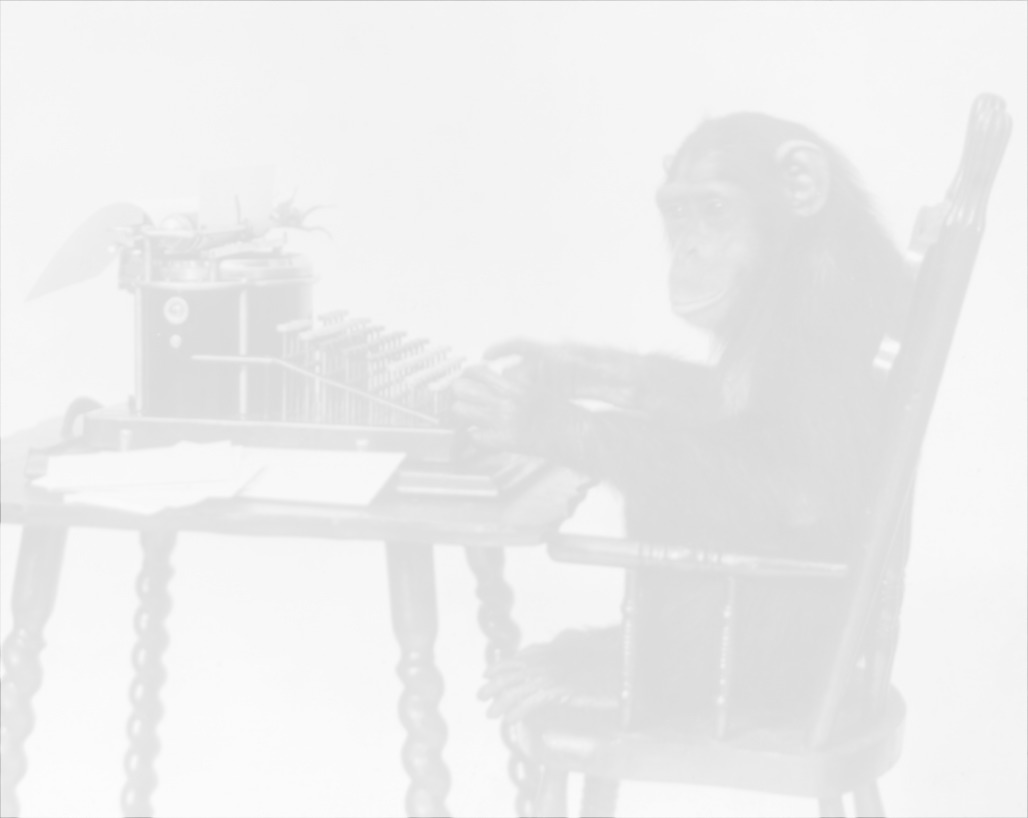
\includegraphics[width=\paperwidth,height=\paperheight]{../../Figures/monkeyTypewriter.jpg}}

% \titlegraphic{\vspace{-7.5mm}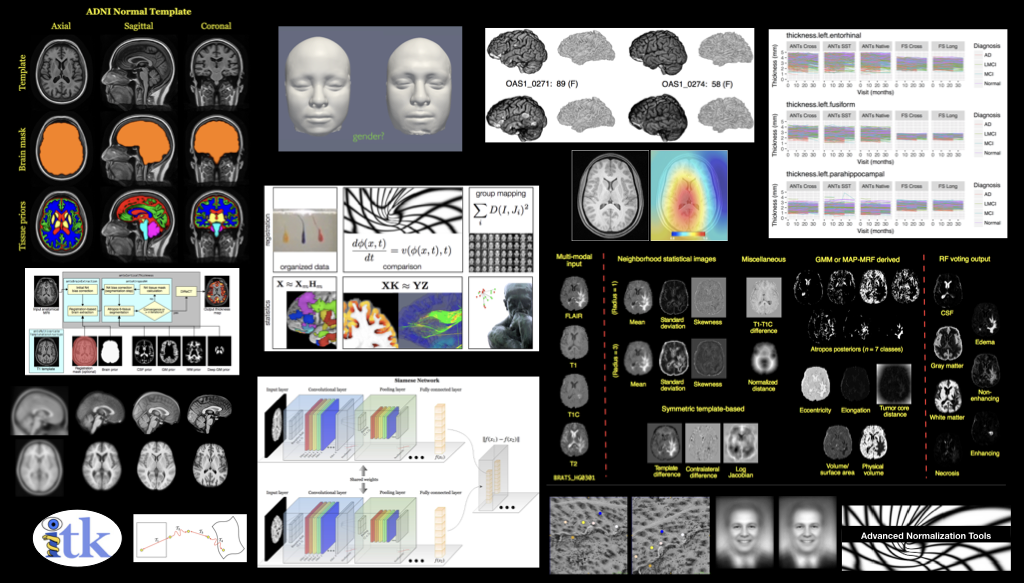
\includegraphics[width=0.45\paperwidth]{../../Figures/montage.png}}

\title{\textbf{Longitudinal mapping of cortical thickness measures}}
\subtitle{\textbf{The ANTs longitudinal cortical thickness pipeline}}
\author{\emph{N. J. Tustison, et al.}}
\date{}

\begin{document}
\frame{\titlepage}

\begin{frame}{ANTs for large-scale neuroimage quantitative analysis}

\vspace*{-.225cm} \hspace*{-.5cm}
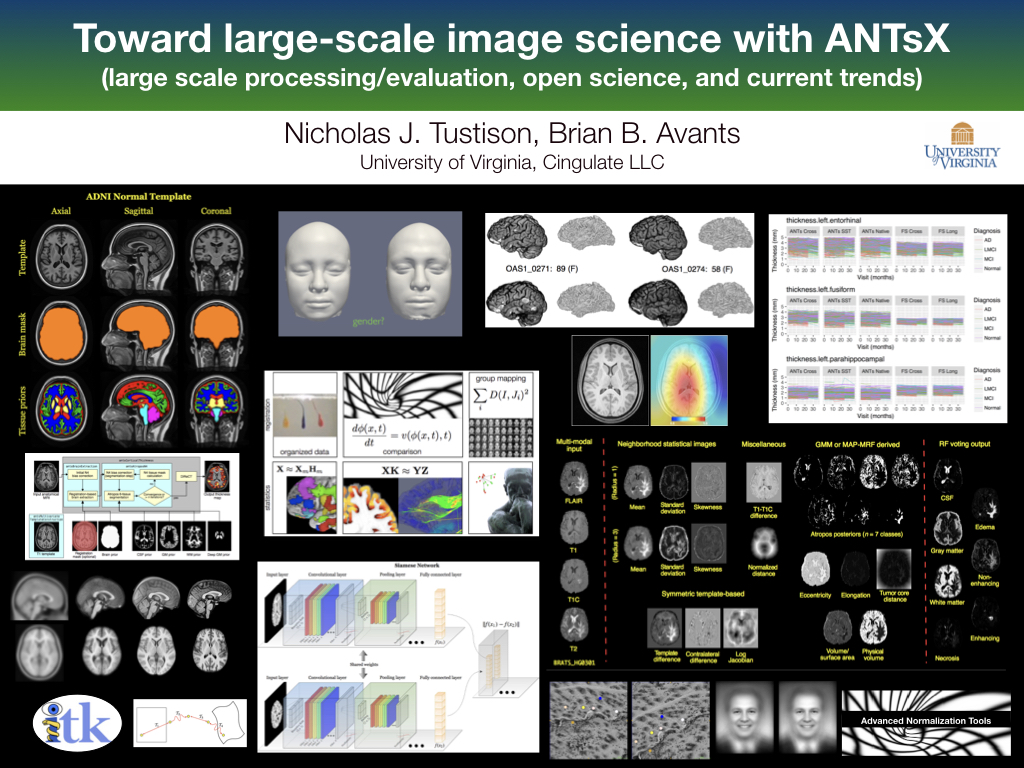
\includegraphics[width=1.07\textwidth,height=0.92\textheight]{../../Figures/montage.pdf}

\end{frame}

\begin{frame}{ANTs open-source ecosystem}

\usebackgroundtemplate{\includegraphics[width=\paperwidth,height=\paperheight]{}}

\vspace*{-.225cm} \hspace*{-.5cm}
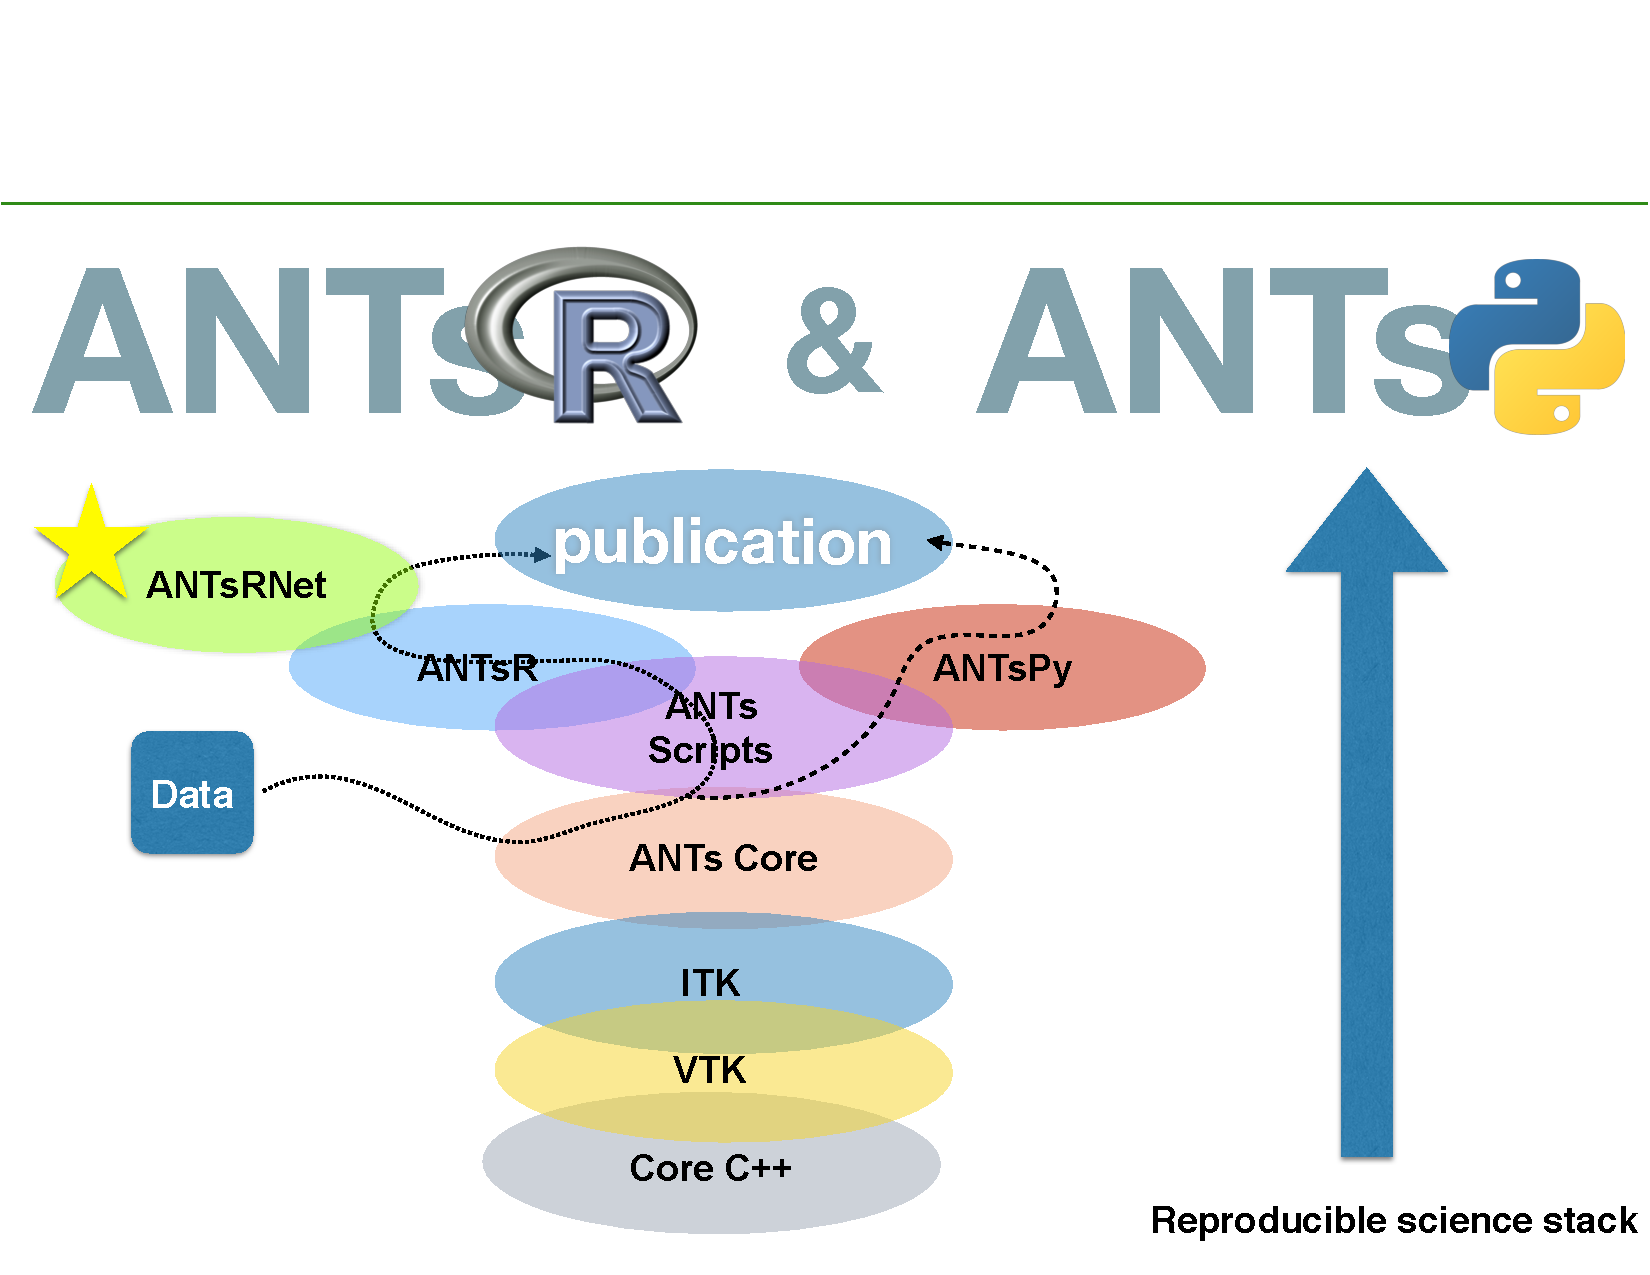
\includegraphics[width=1.07\textwidth,height=0.92\textheight]{../../Figures/antsEcosystem.pdf}

\end{frame}

\begin{frame}{General purpose core}

\vspace*{-.225cm} \hspace*{-.5cm}
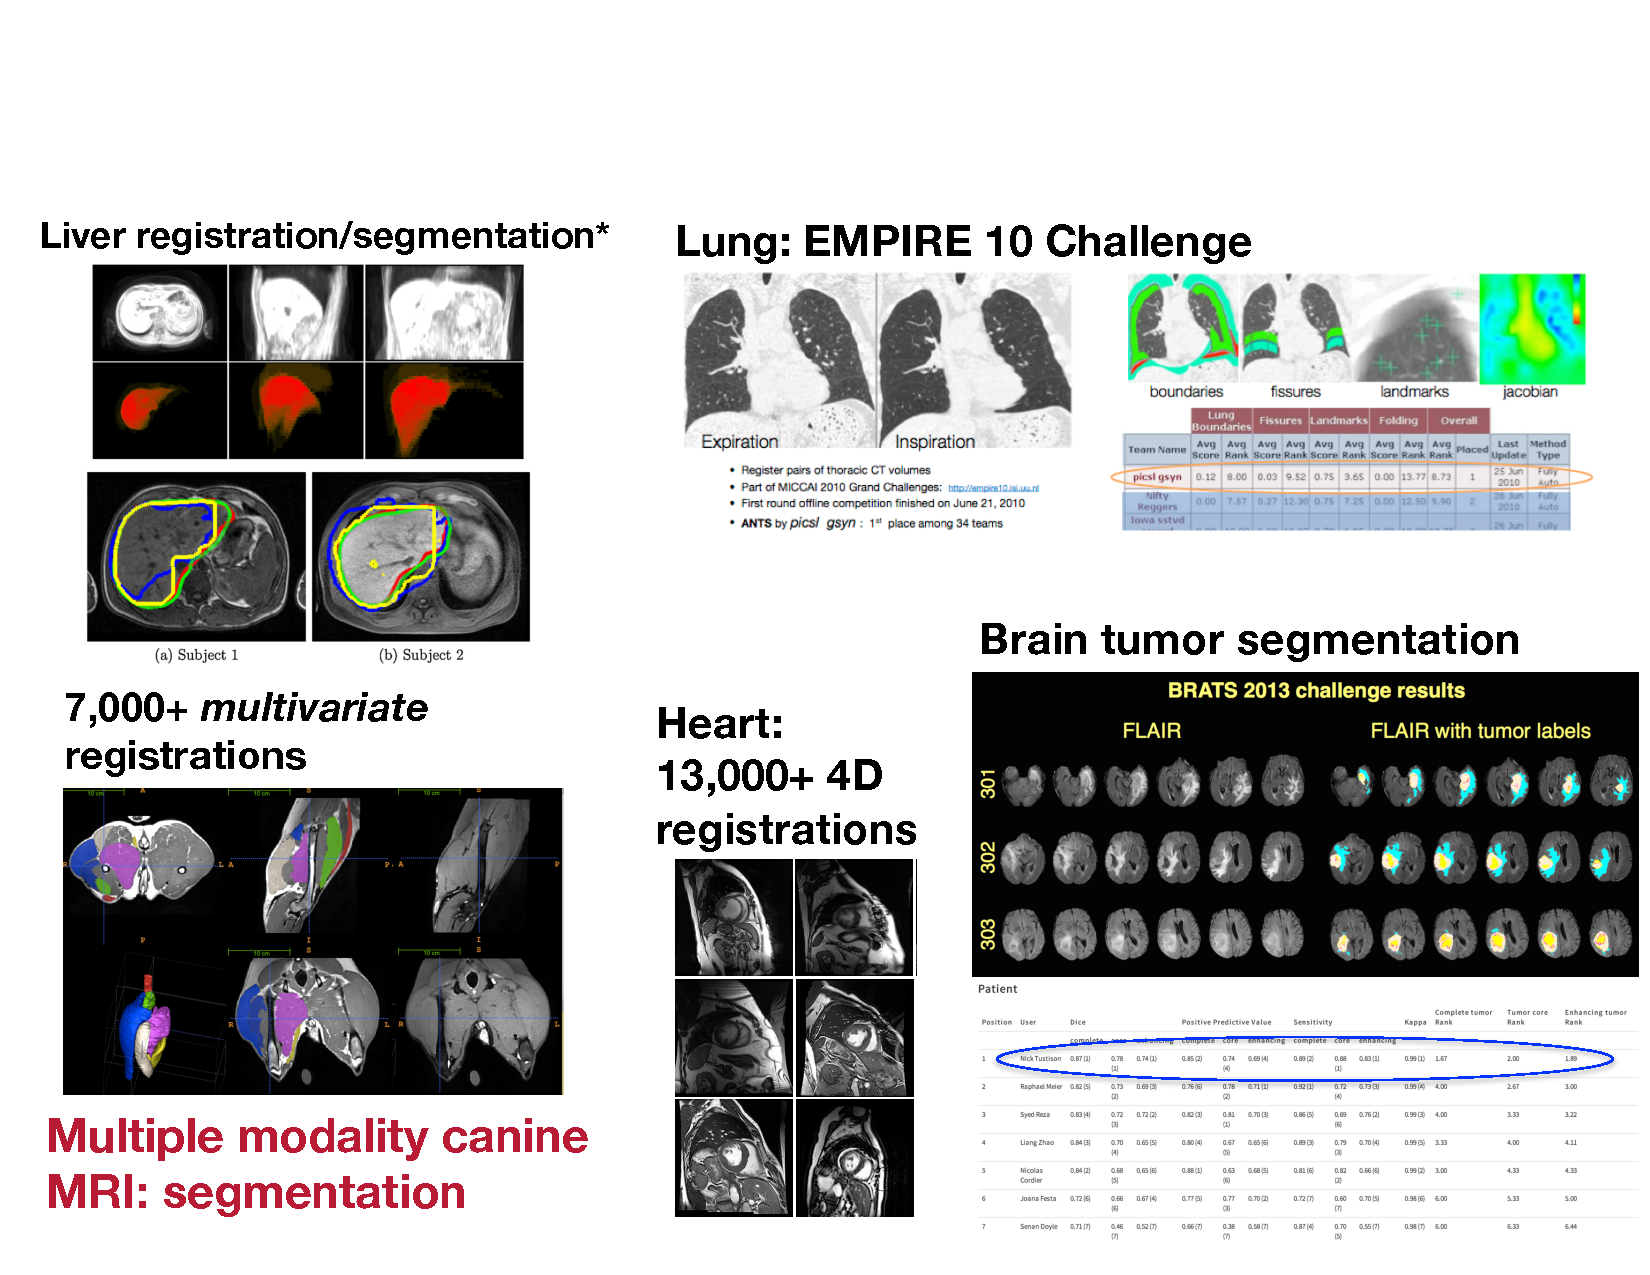
\includegraphics[width=1.07\textwidth,height=0.92\textheight]{../../Figures/antsGeneralPurpose.pdf}

\end{frame}

\begin{frame}{User base (industry and academia)}

\vspace*{-.225cm} \hspace*{-.5cm}

\includegraphics[width=1.07\textwidth,height=0.92\textheight]{../../Figures/userbase.pdf}

\end{frame}

\begin{frame}{DiReCT: cortical thickness}

\usebackgroundtemplate{\includegraphics[width=\paperwidth,height=\paperheight]{}}

\vspace*{-.225cm} \hspace*{-.5cm}
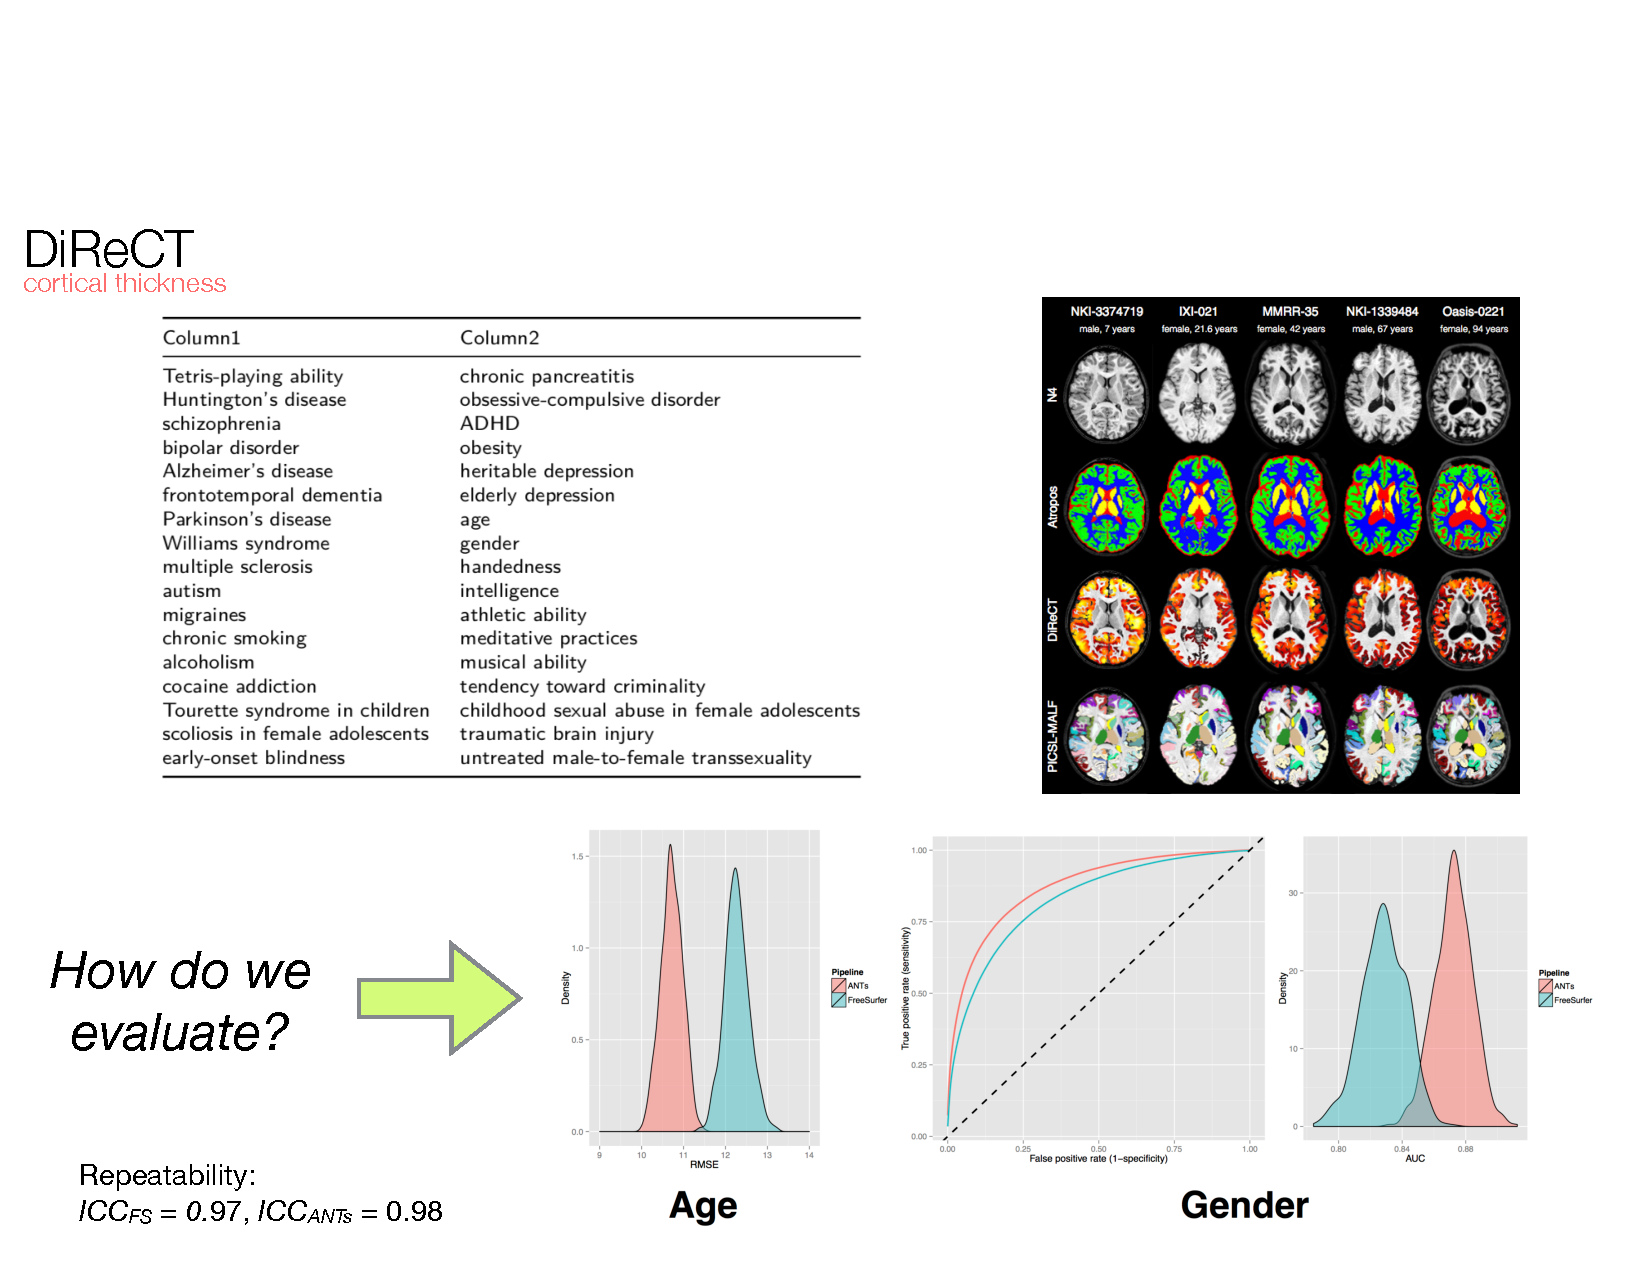
\includegraphics[width=1.085\textwidth,height=0.825\textheight]{../../Figures/direct.pdf}

\tiny

\begin{flushright}
{\em Large-Scale Evaluation of ANTs and FreeSurfer Cortical Thickness Measurements}. NeuroImage, 2014.
\end{flushright}

\end{frame}

\begin{frame}{Cross-sectional comparison}

\centering
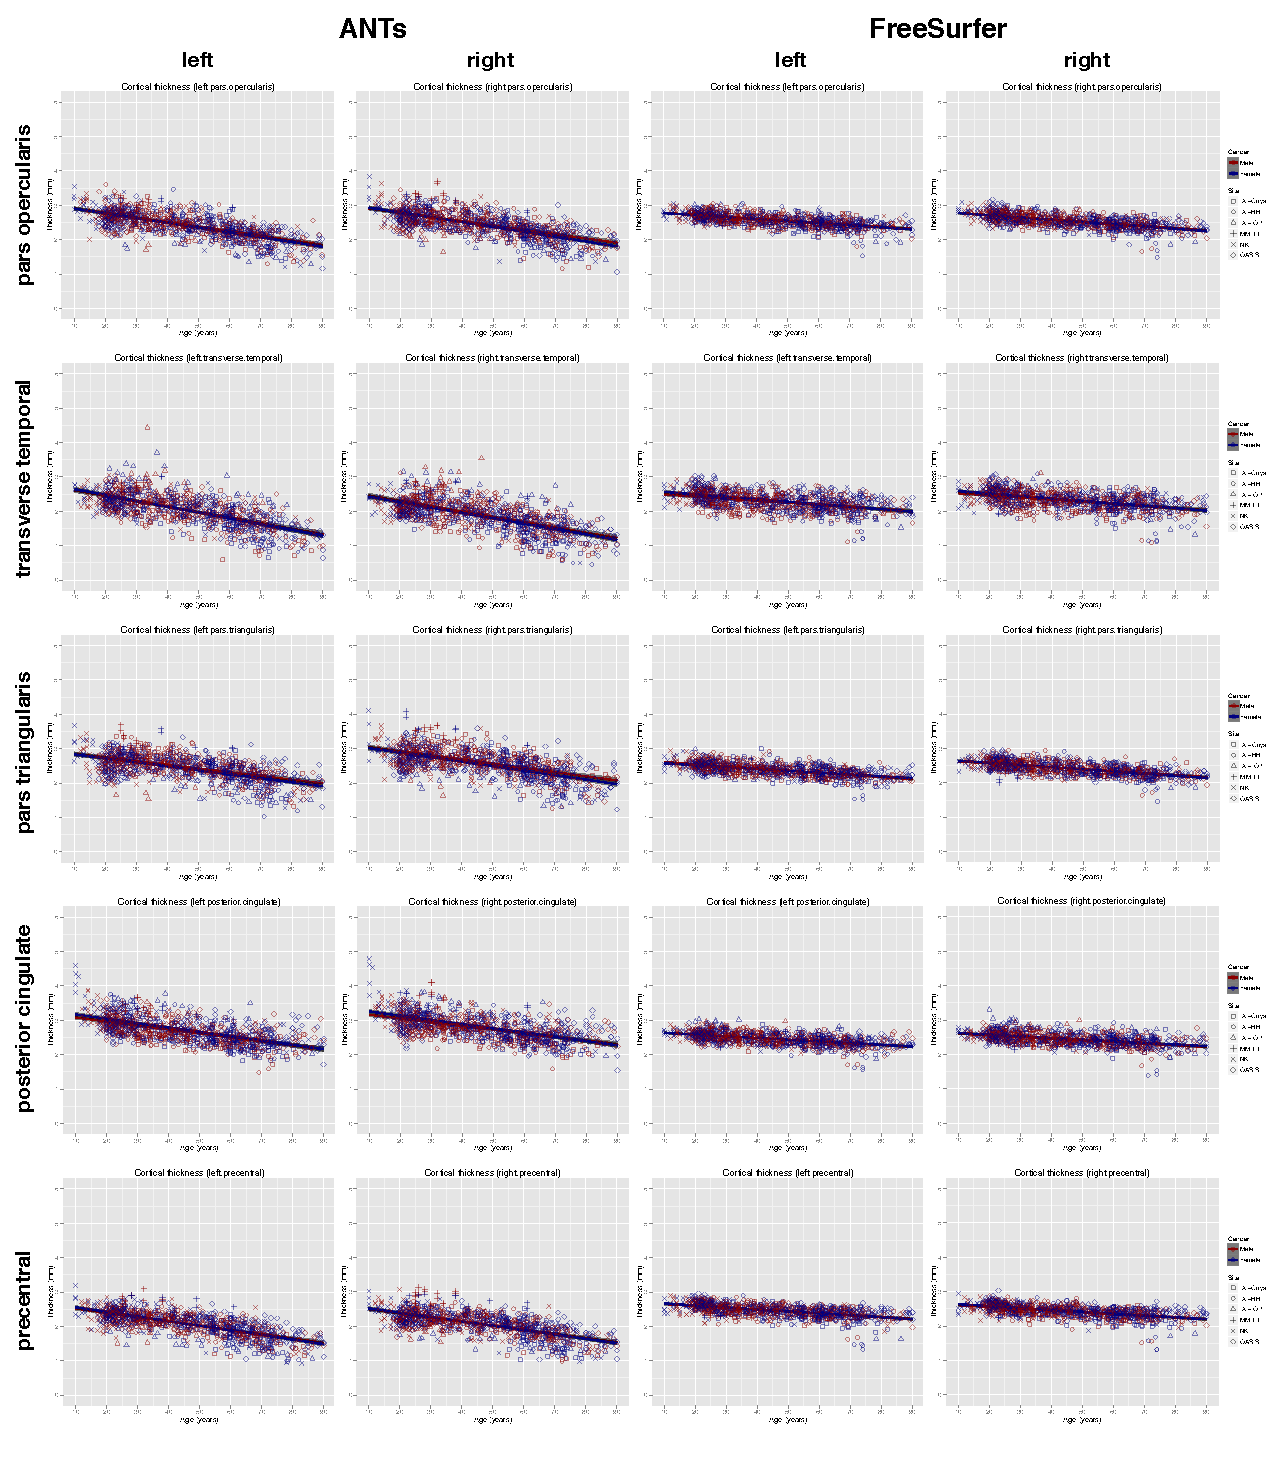
\includegraphics[width=0.99 \textwidth]{../../Figures/rfImportanceRegions.pdf}

\end{frame}

\begin{frame}{FreeSurfer longitudinal pipeline}

\centering
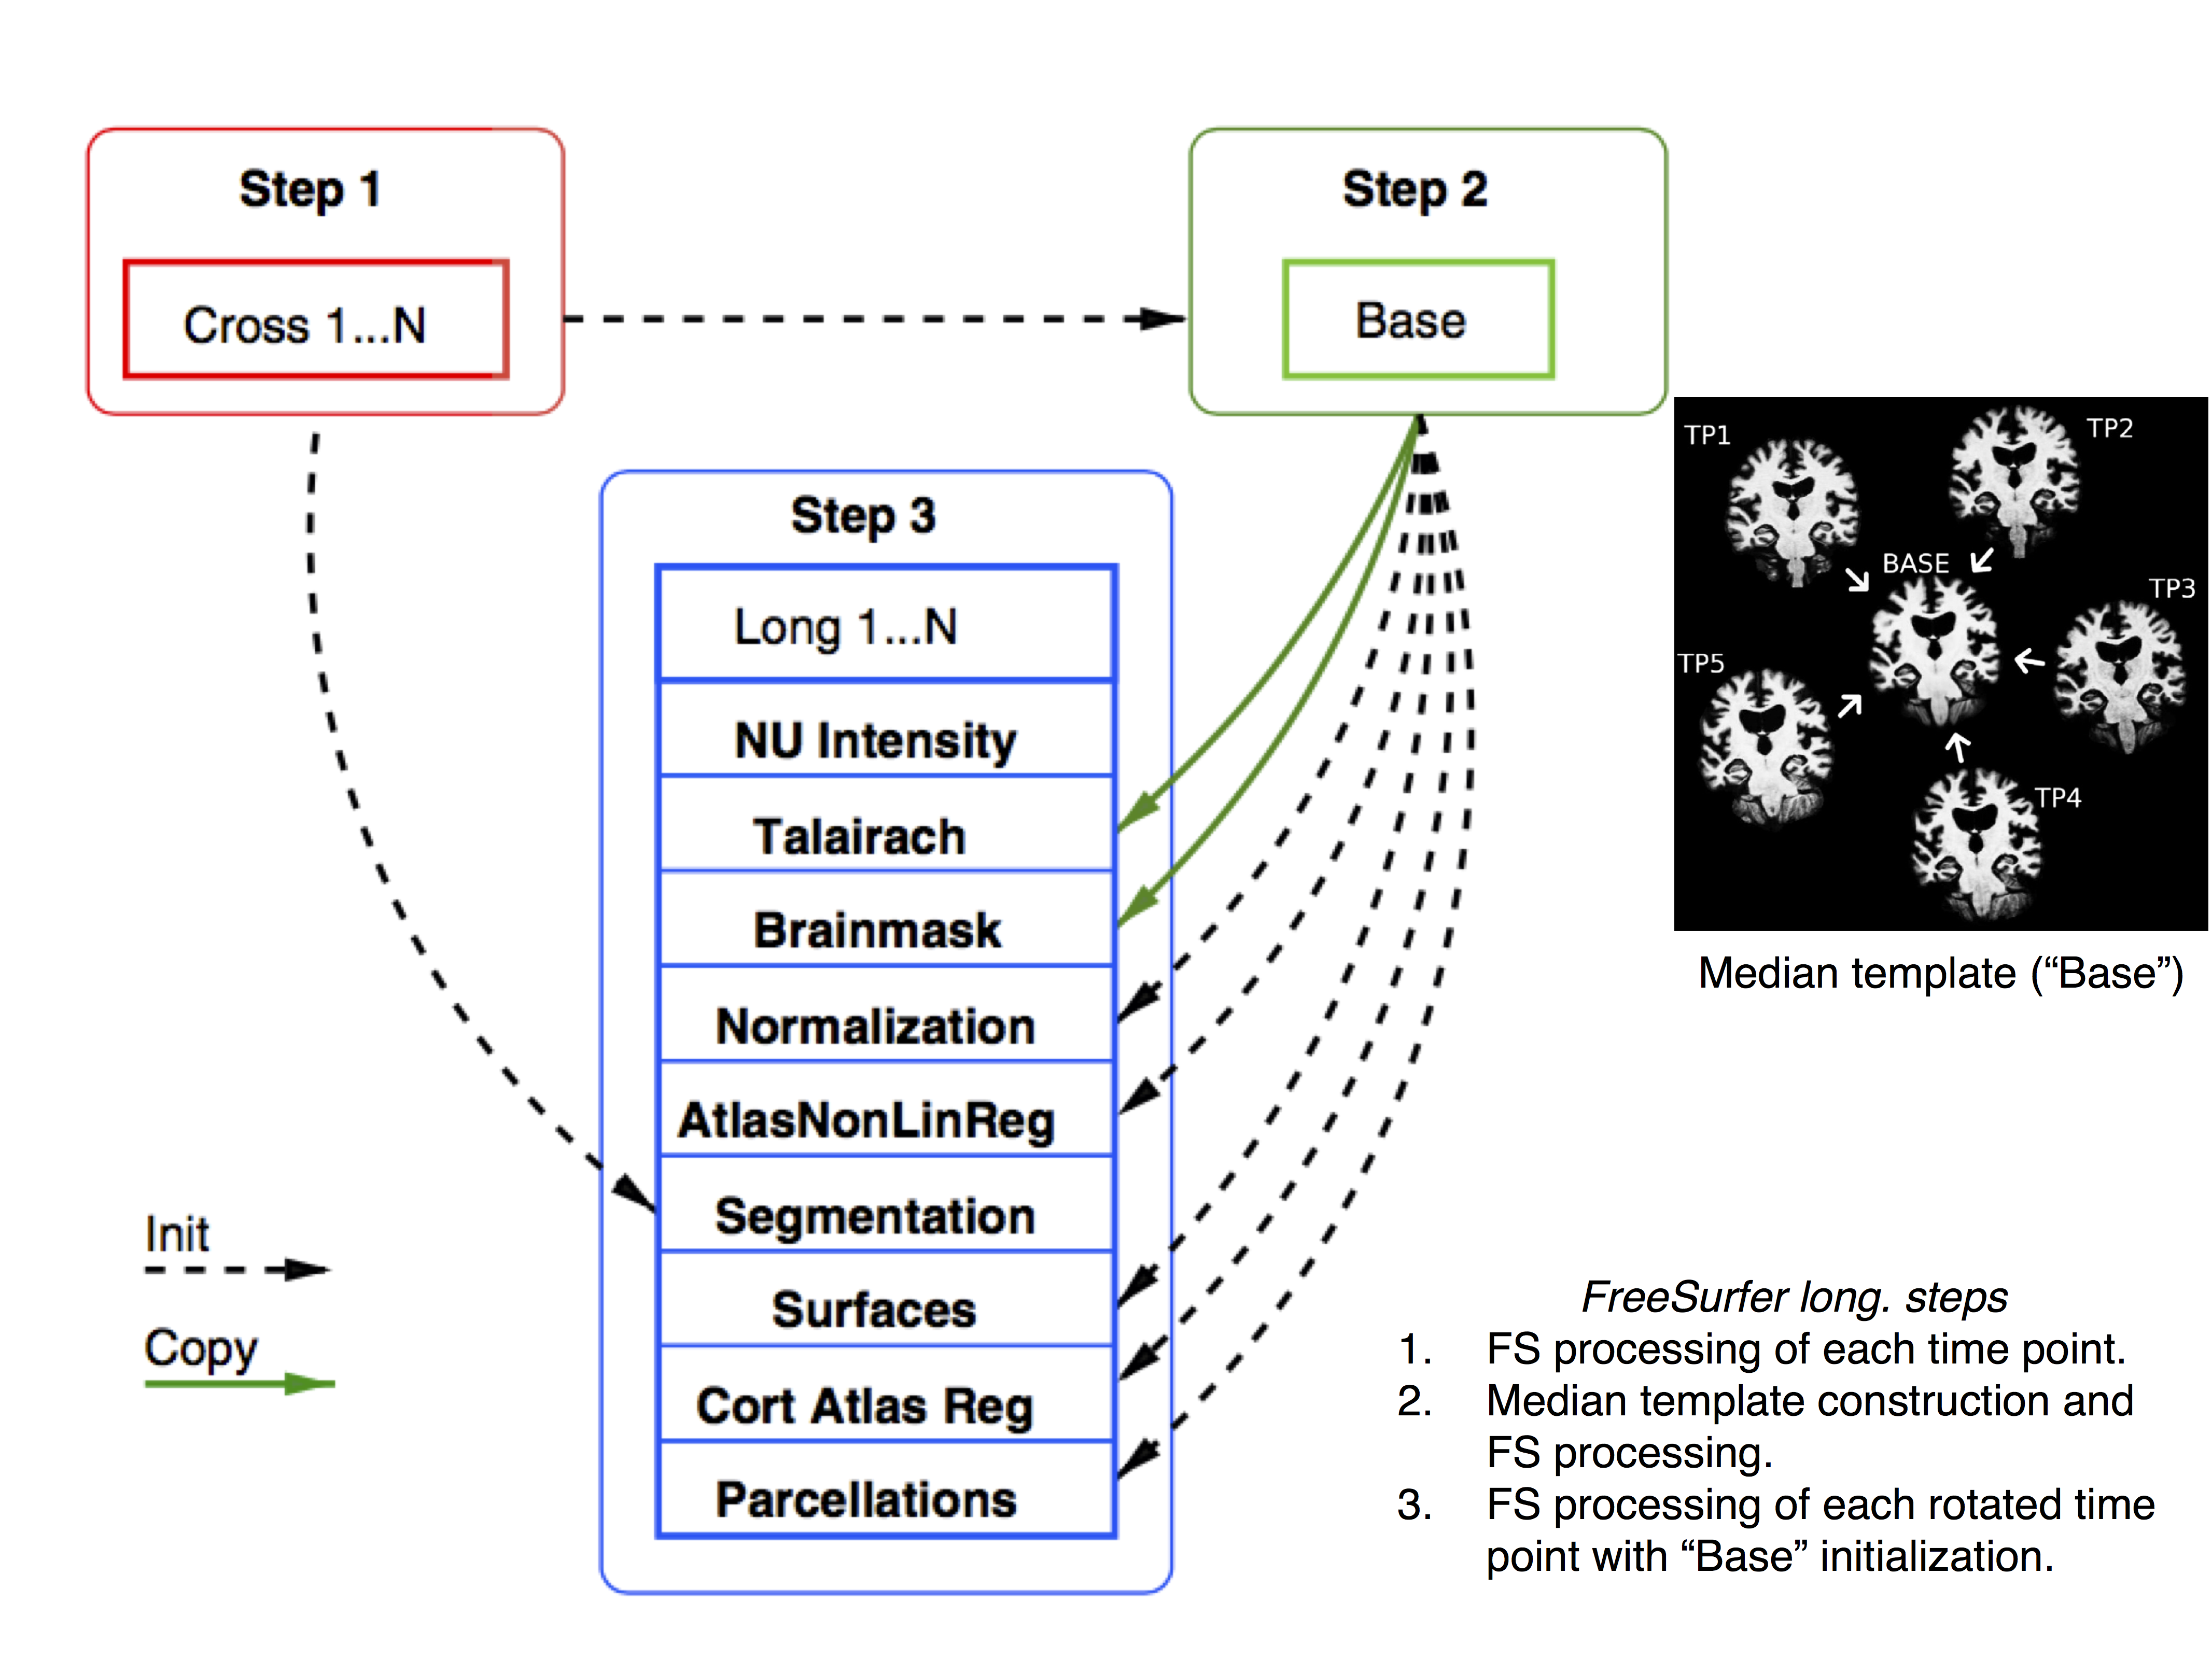
\includegraphics[width=0.85 \textwidth]{../../Figures/FreeSurferLong.png}

\end{frame}

\begin{frame}{ANTs longitudinal pipeline}

\centering
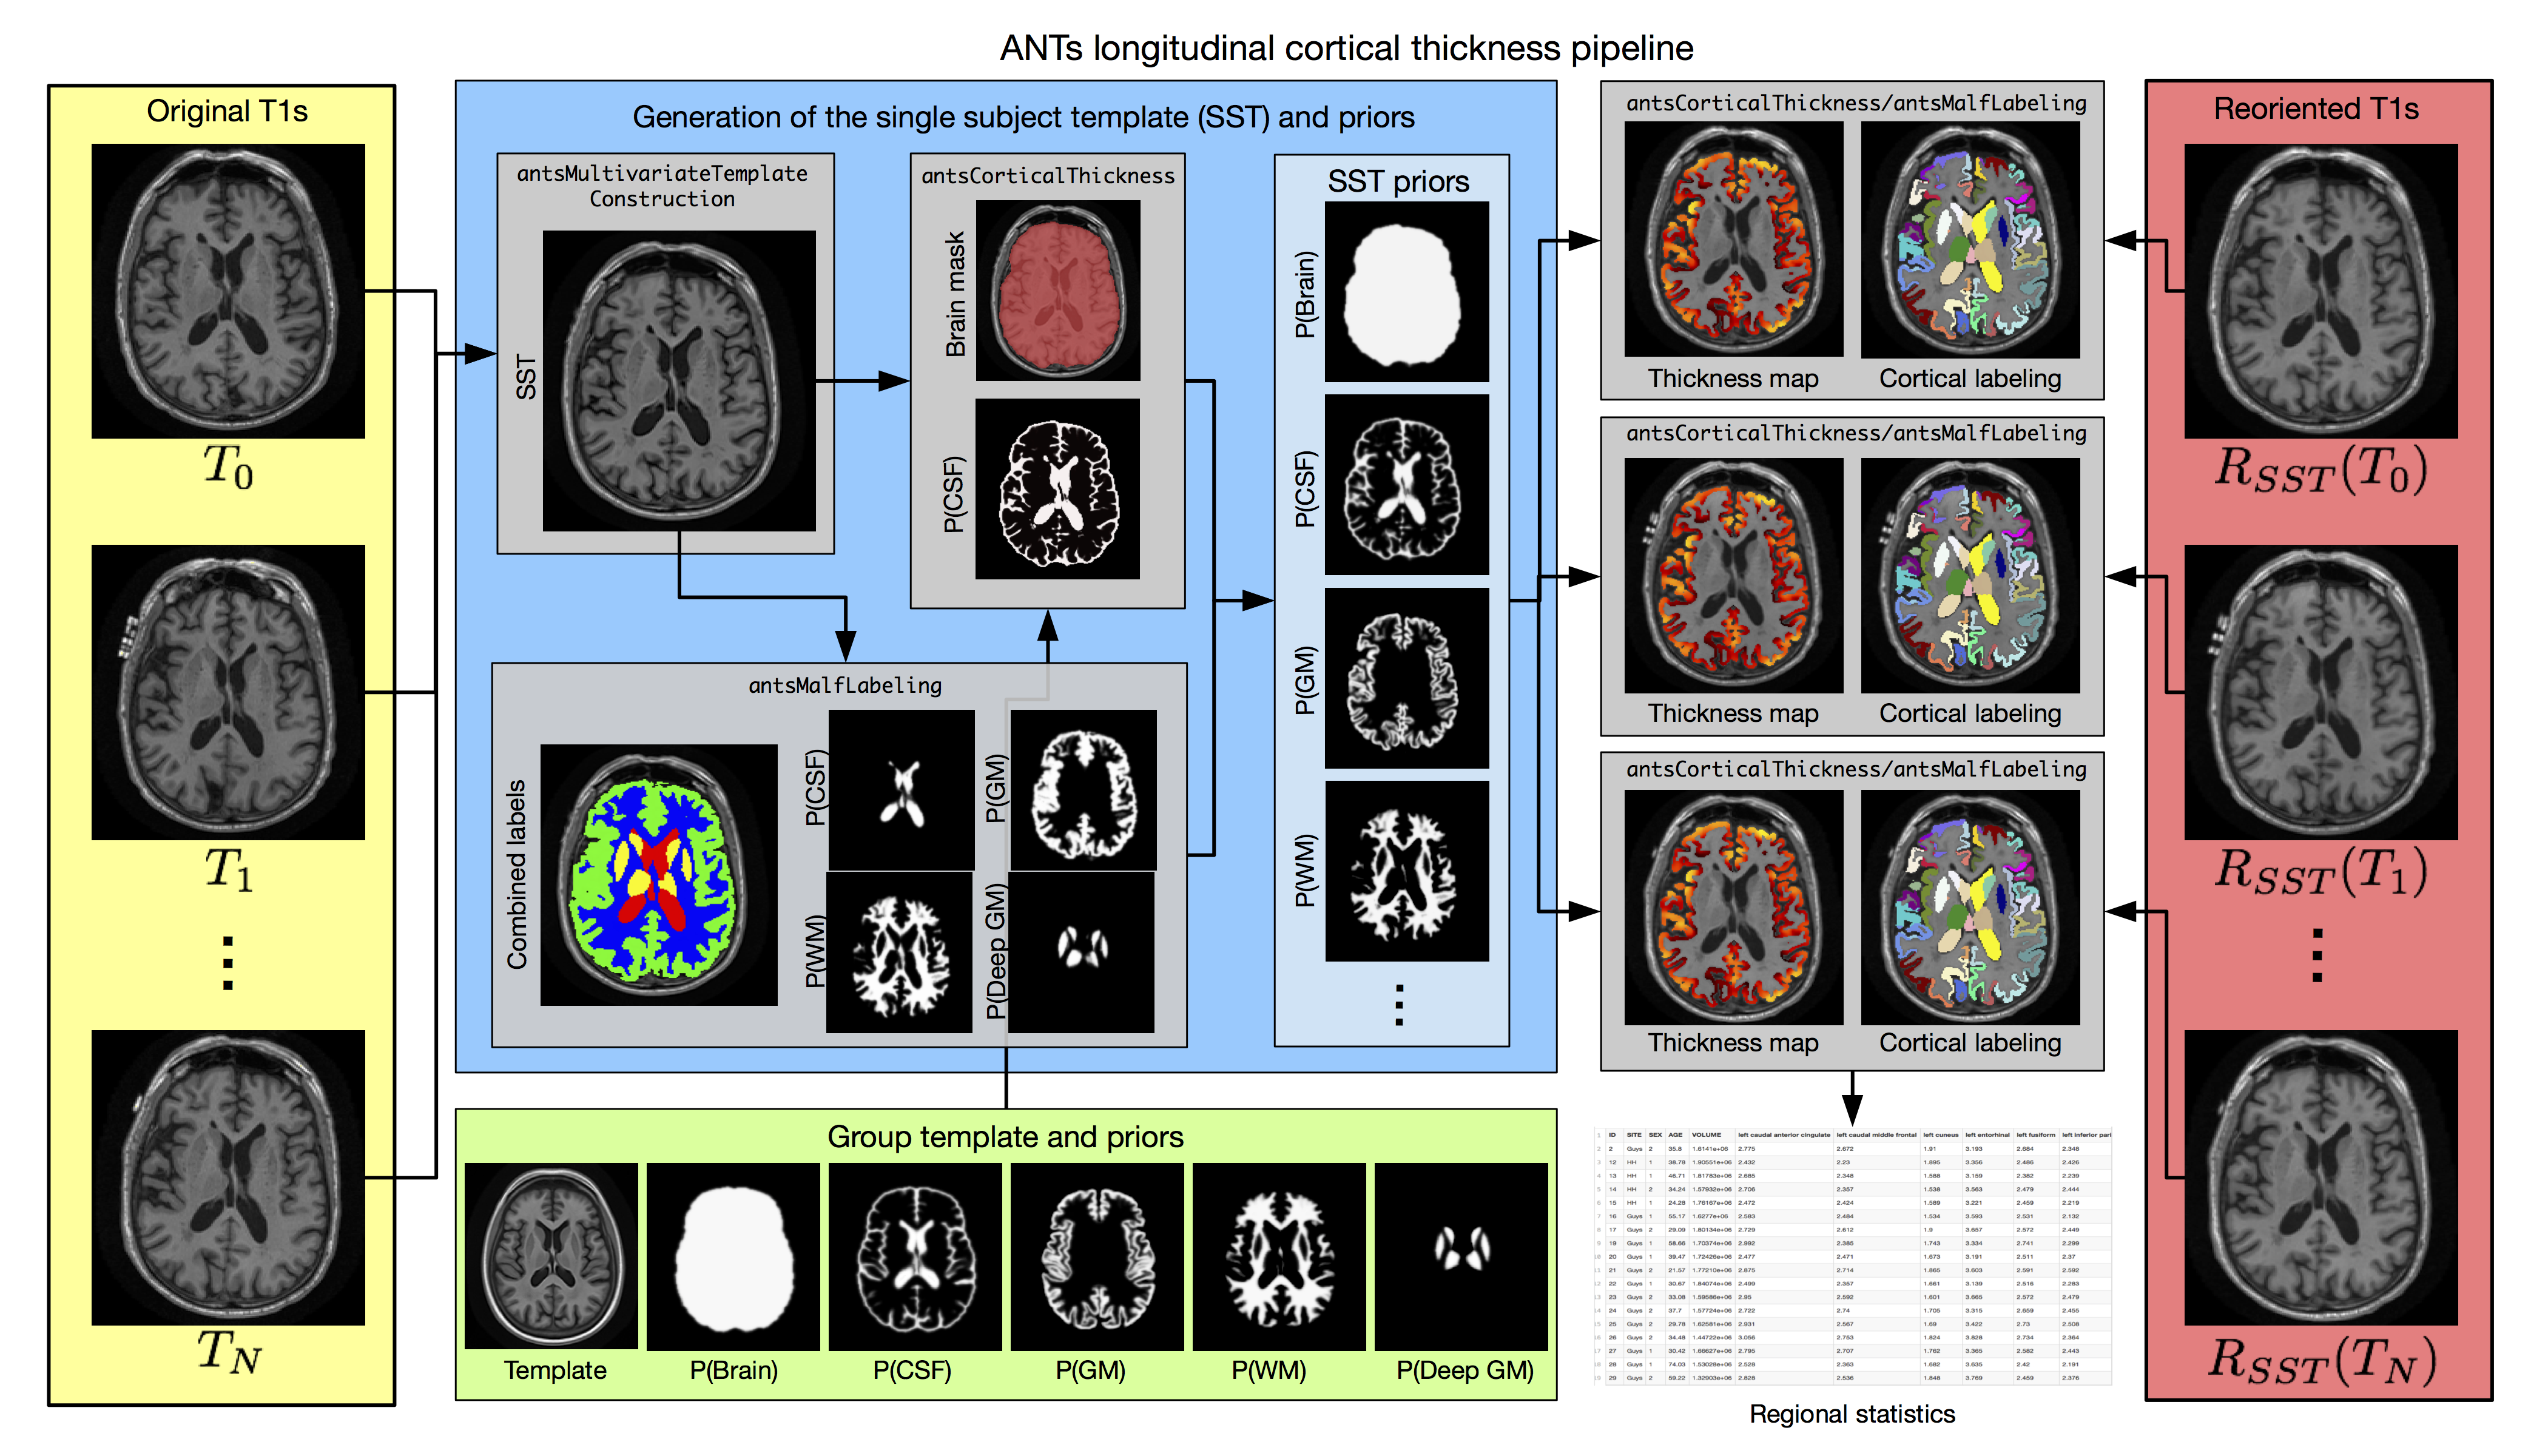
\includegraphics[width=0.99 \textwidth]{../../Figures/longitudinalPipeline.png}

\end{frame}

\end{document}
